%Due to the burgeoning interest in web page speed, there has been a recent rise of network caching literature, tools, and companies.

% TODO(cs): explain that in the NSDI'15 slides, we presented a simple critical
% path model, and
% conjectured that objects on the critical path are often not in cache
% (cacheable). However, we didn't have any evidence for this.

Several papers have analyzed web performance, caching, and the relationship
between CPU speeds and PLT.
% As far as we know, we are the first to jointly isolate all of these factors. % this enables us to easily dissect the effects that caching has on mobile devices.

\textbf{WProf}. Wang et al.~\cite{wang2013demystifying} is the closest research to ours. As we discussed in ~\S\ref{sec:background}, the experiments WProf ran for their Figure 11 show that objects on the critical path are often not cached; and the experiments they ran for their
Figure 13 implies that decreasing CPU speed causes computational delays to comprise a larger fraction of the critical path.

We extend their research along several dimensions.
We develop a model that allows us to predict PLT for a given cache hit ratio. We show that limited RAM does not increase computational delays, though slow CPUs do. We also empirically measure (rather than statically compute, as WProf does) PLTs using a tablet device, and using CPU-constrained virtual machines, over a larger data set (400 URLs, vs. {\footnotesize$\sim$}50 URLs).
Lastly, we extend WProf's cacheability analysis to show that the
marginal returns from caching sharply diminish.

% WProf found that:
%   - Fig 11a & 11b, taken together, seem to imply that objects on the critical
%     path often aren't cached. "cached bytes not proportional to PLT"
%   - Even stronger: Fig 11b shows specifically that while caching reduces 65\%
%     of total object loads, it only reduces 20\% of object loads on the
%     critical path.
%   - Fig 13 seems to imply that decreasing the CPU speed tends to make
%     computational delays dominate over network delays

% Specific ways that we extend their results:
%   - Develop a model, extend their what-if to C=2
%   - Empirically measure slow CPUs, not just what-if. (Fig 7,8,9)
%   - Fig 6 not in WProf (expands on their analysis of K)
%   - Larger dataset: they had at most ~50 URLs, vs. 400 for us.

%\colin{The second and third sentences are too vague.}
\textbf{Web Performance}. Related studies~\cite{web-perf-2, web-perf-3} focus on evaluating and optimizing web performance for desktops. Many techniques such as altering content, data compression, proxy services, and CDNs have been exploited to reduce latency for users. These studies focus on high performing end devices such as desktops. We additionally analyzed web performance on a mobile device and show how this differs from classic desktop environments.
%\jamshed{Say something like `the set of assumptions does not hold for mobile.'}

Zhen Wang et al.~\cite{CPU-plt-2, CPU-plt-3} have determined that the largest delay factor in desktop web page loading is object rendering in the browser. They went further to show that CPU constraints are the lead cause of slow resource loading.
With a large data set, we bolster their claim that CPU constraints are the critical factor in determining page load time. We also demonstrate that web caching has diminishing benefits due to the limited CPU speeds of mobile devices.

We are not the first to focus on web performance for mobile
devices~\cite{CPU-plt-2, CPU-plt-3}.
However, these papers do not explicitly focus on
developing a performance
model for pinpointing the key differences between desktop
and mobile.

%\colin{This is very exciting! If there are papers that claim that caching should help mobile latency, we're showing that they're wrong! We need to emphasize this much more!}
\textbf{Web Caching}. Other literature~\cite{web-caching-1, web-caching-2, web-caching-8, web-caching-9} has focused on the benefits of web caching, specifically the reduction of latency for desktops~\cite{web-caching-3, web-caching-4, web-caching-5, web-caching-6, web-caching-7}.
While these papers make note of the several benefits of caching, they do not
focus on highlighting caching's effects on (CPU-constrained) mobile devices.
% Good.

%Research has also been conducted regarding the correlation between CPU speed and page load times. Jones et al. ~\cite{CPU-plt-1} noted that increased page load time on mobile devices was due to the lack of CPU power, but did not provide backing evidence.

\textbf{Proposed Changes to the Web}. There are many
papers~\cite{web-perf-4-new-design, web-caching-4-new-design,
web-caching-5-new-design, web-caching-latency-1-new-design,
web-caching-latency-2-new-design, web-caching-latency-3-new-design,
web-caching-latency-5-new-design, web-caching-latency-6-new-design,
web-caching-latency-7-new-design} that propose changes to the web that would
improve web latency with better caching schemes. It is possible that under their proposed changes, caching would have more of a benefit for mobile latency. In this paper, we focus only on today's existing infrastructure. % We further show that increasing the hit ratio of caches only provides marginal benefits to mobile page load time.

%\jamshed{TODO: discuss other methodologies, why is our apparatus novel?}
% \jamshed{From Colin: Most other papers measure results "in the wild", i.e. on real networks. That's useful for the final results, but it's hard to control it well enough to get repeatable results.}
%\begin{figure}[t]
%    %\hspace{-10pt}
%    \figuretitle{Fraction Reduction in PLT with Inflated Delays}
%    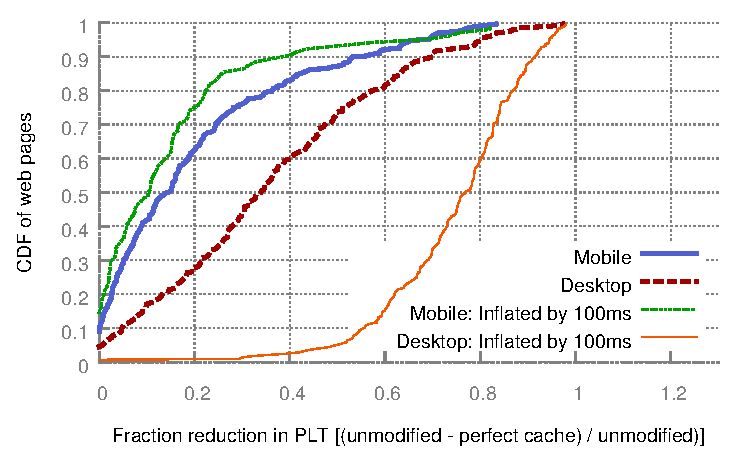
\includegraphics[width=3in]{../graphs/percent_plt_reduction/percent_reduction_linear_inflated.pdf}
%    \caption[]{\label{fig:inflated_delays}In networks with high latency, caching has a negligible effect on mobile PLTs, but a significant benefit for desktop PLTs.}
    % Just remove the first sentence of the caption?
%\end{figure}

